\documentclass[12pt]{article}
\usepackage{a4wide}
\usepackage{color, amssymb}
\usepackage[margin=1in]{geometry}
\usepackage[document]{ragged2e}
\usepackage[table]{xcolor}
\usepackage{multirow}
\usepackage[braket, qm]{qcircuit}
\setlength{\arrayrulewidth}{0.5mm}
\setlength{\tabcolsep}{16pt}
\renewcommand{\arraystretch}{1.9}
\usepackage[english,greek]{babel}
\usepackage{braket}
\usepackage{mathtools}
\usepackage{ragged2e}
\renewcommand{\baselinestretch}{1.5}
\input{epsf}
\usepackage{float}
\usepackage{graphicx}
\usepackage{caption}
\usepackage{subcaption}
\usepackage{cancel}
\usepackage{algorithm}
\usepackage{animate}
\usepackage[noend]{algpseudocode}

\begin{document}

\greektext

\noindent\rule{\textwidth}{2pt}
\begin{center}
{\bf ΚΒΑΝΤΙΚΗ ΤΕΧΝΟΛΟΓΙΑ}\\ 
{\bf 2o Σετ Ασκήσεων }\\
{\bf Καλαμαράκης Θεόδωρος:} 2018030022\\
\end{center}
\rule{\textwidth}{.5pt}
\noindent

\begin{center}

\end{center}
 
 

\justifying




%%%%%%%%%%%%%%%%%%%%%%%%%%%%%%%%%%%%%%%%%%%%%%%%%%%%%%%%%%%%%%%%%%%%%%%%%%%%%%%%%%%%%%%%%%%%%%%%%%%%%%%%%%%%%%%%%%%%%%%%%%%%%%%%%%%%%%%
\section*{{\bfΆσκηση 1}}
Εφαρμόζοντας την σχέση $(1.13)$ διαδοχικά για όλες τις ιδιοκαταστάσεις απο $\ket{0}$ μέχρι $\ket{n}$ έχουμε 

$$
\begin{array}{lr}
\ket{n}= \frac{\alpha^\dag}{\sqrt{n}}\ket{n-1}\\
\ket{n-1}= \frac{\alpha^\dag}{\sqrt{n-1}}\ket{n-2}\\
\vdots\\
\ket{1}= \frac{\alpha^\dag}{\sqrt{1}}\ket{0}\\
\end{array}
$$
πολλαπλασιάζοντας κατα μέλη παίρνουμε:
$$
\left\{
\begin{array}{lr}
\ket{n}= \frac{\alpha^\dag}{\sqrt{n}}\cancelto{}{ \ket{n-1}}\\
\cancelto{}{\ket{n-1}}= \frac{\alpha^\dag}{\sqrt{n-1}}\cancelto{}{\ket{n-2}}\\
\vdots\\
\cancelto{}{\ket{1}}= \frac{\alpha^\dag}{\sqrt{1}}\ket{0}\\
\end{array}
\right\} \Rightarrow \ket{n} = \frac{\alpha^\dag \cdot \alpha^\dag\cdot \hdots\cdot \alpha^\dag }{\sqrt{n}\cdot \sqrt{n-1}\cdot \hdots \cdot \sqrt{1}}\ket{0} \Leftrightarrow
$$
$$\Leftrightarrow \ket{n} = \frac{\left(\alpha^\dag\right)^n}{\sqrt{n!}}\ket{0}$$
\rule{\textwidth}{.5pt}
\section*{{\bfΆσκηση 2}}
\underline{Για την μέση τιμή της θέσης} \\
$$\braket{x}_t = \bra{\psi(t)}x \ket{\psi(t)} $$
όπου $x = x_0(\alpha^\dag+\alpha)$, $x_0 = \sqrt{\frac{\hbar}{2m\omega}}$ και 
$$ \psi(t) =e^{-\frac{iHt}{\hbar}}\psi(0) = e^{-\frac{iHt}{\hbar}}\left(\frac{1}{\sqrt{3}}\ket{0}+\frac{2}{\sqrt{3}}\ket{2}\right)$$
Για τη Χαμιλτονινή μπορούμε να γράψουμε 
$$H = \left(\frac{1}{2}\right)\hbar\omega\ket{0}\bra{0}+\left(1+\frac{1}{2}\right)\hbar\omega\ket{1}\bra{1}+\hdots+\left(n+\frac{1}{2}\right)\hbar\omega\ket{n}\bra{n} = \sum_{j=0}^n\left(j+\frac{1}{2}\right)\hbar\omega\ket{j}\bra{j}$$
Αρα
$$e^{-\frac{iHt}{\hbar}} = \sum_{j=0}^n e^{-\frac{i\left(\left(j+\frac{1}{2}\right)\hbar\omega\right)t}{\hbar}}\ket{j}\bra{j} =  \sum_{j=0}^n e^{-i\left(j+\frac{1}{2}\right)\omega t}\ket{j}\bra{j}$$
Αρα 
\begin{align*}
\psi(t) &= e^{-\frac{iHt}{\hbar}}\left(\frac{1}{\sqrt{3}}\ket{0}+\frac{2}{\sqrt{3}}\ket{2}\right) = \sum_{j=0}^n e^{-i\left(j+\frac{1}{2}\right)\omega t}\ket{j}\bra{j}\left(\frac{1}{\sqrt{3}}\ket{0}+\frac{2}{\sqrt{3}}\ket{2}\right) =\\
&=\frac{1}{\sqrt{3}}e^{-i\frac{1}{2}\omega t}\ket{0}+\frac{2}{\sqrt{3}}e^{-i\frac{5}{2}\omega t}\ket{2}
\end{align*}
Συνεπώς 
\begin{align*}
    x\ket{\psi(t)} &= x_0\left(\alpha^\dag +\alpha \right)\left(\frac{1}{\sqrt{3}}e^{-i\frac{1}{2}\omega t}\ket{0}+\frac{2}{\sqrt{3}}e^{-i\frac{5}{2}\omega t}\ket{2}\right) =  \\
    &=x_0\left(\cancelto{0}{\frac{1}{\sqrt{3}}e^{-i\frac{1}{2}\omega t}\alpha\ket{0}} + \frac{1}{\sqrt{3}}e^{-i\frac{1}{2}\omega t}\alpha^\dag\ket{0}+\frac{2}{\sqrt{3}}e^{-i\frac{5}{2}\omega t}\alpha\ket{2}+\frac{2}{\sqrt{3}}e^{-i\frac{5}{2}\omega t}\alpha^\dag\ket{2}\right)=\\
    &= x_0\left(\left(\frac{1}{\sqrt{3}}e^{-i\frac{1}{2}\omega t}+\frac{2}{\sqrt{3}}e^{-i\frac{5}{2}\omega t}\right)\ket{1} + \frac{2}{\sqrt{3}}e^{-i\frac{5}{2}\omega t}\ket{3}\right)
\end{align*}
Αρα 
\begin{align*}
    \braket{x}_t &= \bra{\psi(t)}x\ket{\psi(t)} =\\
    &= x_0\left(\frac{1}{\sqrt{3}}e^{i\frac{1}{2}\omega t}\bra{0}+\frac{2}{\sqrt{3}}e^{i\frac{5}{2}\omega t}\bra{2}\right)\left(\left(\frac{1}{\sqrt{3}}e^{-i\frac{1}{2}\omega t}+\frac{2}{\sqrt{3}}e^{-i\frac{5}{2}\omega t}\right)\ket{1} + \frac{2}{\sqrt{3}}e^{-i\frac{5}{2}\omega t}\ket{3}\right)=0   
\end{align*}\\
\underline{Για την μέση τιμή της ορμής} \\
$$\braket{p}_t = \bra{\psi(t)}p \ket{\psi(t)} $$
όπου $p = p_0(\alpha^\dag-\alpha)$ και $p_0 = i\sqrt{\frac{m\omega\hbar}{2}}$ \\
Συνεπώς 
\begin{align*}
    p\ket{\psi(t)} &= p_0\left(\alpha^\dag -\alpha \right)\left(\frac{1}{\sqrt{3}}e^{-i\frac{1}{2}\omega t}\ket{0}+\frac{2}{\sqrt{3}}e^{-i\frac{5}{2}\omega t}\ket{2}\right) =  \\
    &=p_0\left(-\cancelto{0}{\frac{1}{\sqrt{3}}e^{-i\frac{1}{2}\omega t}\alpha\ket{0}} + \frac{1}{\sqrt{3}}e^{-i\frac{1}{2}\omega t}\alpha^\dag\ket{0}-\frac{2}{\sqrt{3}}e^{-i\frac{5}{2}\omega t}\alpha\ket{2}+\frac{2}{\sqrt{3}}e^{-i\frac{5}{2}\omega t}\alpha^\dag\ket{2}\right)=\\
    &= p_0\left(\left(\frac{1}{\sqrt{3}}e^{-i\frac{1}{2}\omega t}-\frac{2}{\sqrt{3}}e^{-i\frac{5}{2}\omega t}\right)\ket{1} + \frac{2}{\sqrt{3}}e^{-i\frac{5}{2}\omega t}\ket{3}\right)
\end{align*}
Αρα 
\begin{align*}
    \braket{p}_t &= \bra{\psi(t)}p\ket{\psi(t)} =\\
    &= p_0\left(\frac{1}{\sqrt{3}}e^{i\frac{1}{2}\omega t}\bra{0}+\frac{2}{\sqrt{3}}e^{i\frac{5}{2}\omega t}\bra{2}\right)\left(\left(\frac{1}{\sqrt{3}}e^{-i\frac{1}{2}\omega t}+\frac{2}{\sqrt{3}}e^{-i\frac{5}{2}\omega t}\right)\ket{1} + \frac{2}{\sqrt{3}}e^{-i\frac{5}{2}\omega t}\ket{3}\right)=0   
\end{align*}\\
Για τις αβεβαιότητες έχουμε
\begin{align*}
    \Delta X = \sqrt{\braket{x^2}- \braket{x}^2} = \sqrt{\braket{x^2}} = 
\end{align*}
\begin{align*}
    \braket{x^2} &= \bra{\psi(t)}x^2\ket{\psi(t)} = x_0^2 e^{\frac{iHt}{\hbar}}\bra{\psi(0)}\left(\alpha \alpha +\alpha^\dag\alpha^\dag + \alpha^\dag \alpha +\alpha \alpha^\dag\right)e^{-\frac{iHt}{\hbar}}\ket{\psi(0)} = \\
    &=x_0^2 \bra{\psi(0)}\left( \alpha^\dag \alpha +\alpha \alpha^\dag\right)\ket{\psi(0)} = x_0^2\bra{\psi(0)}\left(\cancelto{0}{\alpha^\dag \alpha\frac{1}{\sqrt{3}}\ket{0}}+\alpha \alpha^\dag\frac{1}{\sqrt{3}}\ket{0} +\alpha^\dag \alpha\frac{\sqrt{2}}{\sqrt{3}}\ket{2}+\alpha \alpha^\dag\frac{\sqrt{2}}{\sqrt{3}}\ket{2} \right)\\
    &=x_0^2\bra{\psi(0)}\left(\frac{1}{\sqrt{3}}\ket{0} +2\frac{\sqrt{2}}{\sqrt{3}}\ket{2}+3\frac{\sqrt{2}}{\sqrt{3}}\ket{2} \right) = x_0^2\left(\frac{1}{\sqrt{3}}\bra{0} +\frac{\sqrt{2}}{\sqrt{3}}\bra{2} \right)\left(\frac{1}{\sqrt{3}}\ket{0} +5\frac{\sqrt{2}}{\sqrt{3}}\ket{2} \right)\\
    &=\frac{\hbar}{2m\omega}\left(\frac{1}{3}+ 5\frac{2}{3}\right) = \frac{11\hbar}{6m\omega}
\end{align*}
Ara $$\Delta X = \sqrt{\frac{11\hbar}{6m\omega}}$$
\begin{align*}
    \Delta P = \sqrt{\braket{p^2}- \braket{p}^2} = \sqrt{\braket{p^2}} = 
\end{align*}
\begin{align*}
    \braket{p^2} &= \bra{\psi(t)}p^2\ket{\psi(t)} = p_0^2 e^{\frac{iHt}{\hbar}}\bra{\psi(0)}\left(\alpha \alpha +\alpha^\dag\alpha^\dag - \alpha^\dag \alpha -\alpha \alpha^\dag\right)e^{-\frac{iHt}{\hbar}}\ket{\psi(0)} = \\
    &=-p_0^2 \bra{\psi(0)}\left( \alpha^\dag \alpha +\alpha \alpha^\dag\right)\ket{\psi(0)} = p_0^2\bra{\psi(0)}\left(\cancelto{0}{\alpha^\dag \alpha\frac{1}{\sqrt{3}}\ket{0}}+\alpha \alpha^\dag\frac{1}{\sqrt{3}}\ket{0} +\alpha^\dag \alpha\frac{\sqrt{2}}{\sqrt{3}}\ket{2}+\alpha \alpha^\dag\frac{\sqrt{2}}{\sqrt{3}}\ket{2} \right)\\
    &=-p_0^2\bra{\psi(0)}\left(\frac{1}{\sqrt{3}}\ket{0} +2\frac{\sqrt{2}}{\sqrt{3}}\ket{2}+3\frac{\sqrt{2}}{\sqrt{3}}\ket{2} \right) = p_0^2\left(\frac{1}{\sqrt{3}}\bra{0} +\frac{\sqrt{2}}{\sqrt{3}}\bra{2} \right)\left(\frac{1}{\sqrt{3}}\ket{0} +5\frac{\sqrt{2}}{\sqrt{3}}\ket{2} \right)\\
    &=\frac{m\omega\hbar}{2}\left(\frac{1}{3}+ 5\frac{2}{3}\right) = \frac{11m\omega\hbar}{6}
\end{align*}
Ara $$\Delta P = \sqrt{\frac{11m\omega\hbar}{6}}$$
\rule{\textwidth}{.5pt}
\section*{{\bfΆσκηση 3}}
Απο την σχέση $ \ket{n} = \frac{\left(\alpha^\dag\right)^n}{\sqrt{n!}}\ket{0}$ προκύπτει οτι 
$$ \psi_n(x) = \braket{x|n} =\frac{1}{\sqrt{n!2^n}}\left[\sqrt{m\omega}x - \frac{1}{\sqrt{m \omega}}\frac{d}{dx} \right]^n\psi_0(x)$$
\begin{itemize}
    \item για $n=1$ 
        $$\psi_1(x) = \frac{1}{\sqrt{2}}\left[\sqrt{m\omega}x - \frac{1}{\sqrt{m \omega}}\frac{d}{dx} \right]\psi_0(x)\Leftrightarrow$$
        $$\psi_1(x) =\frac{1}{\sqrt{2}}\left[\sqrt{m\omega}x - \frac{1}{\sqrt{m \omega}}\frac{d}{dx} \right] ke^{-m\omega x^2/2}\Leftrightarrow$$
        $$\psi_1(x) =\frac{1}{\sqrt{2}}k\left[\sqrt{m\omega}xe^{-m\omega x^2/2} + \sqrt{m \omega}xe^{-m\omega x^2/2} \right]  = k\sqrt{2m\omega}xe^{-m\omega x^2/2}$$
        Για να είναι η $\psi_1(x)$ κανονικοποιήμενη πρέπει $\int_{-\infty}^{+\infty}|\psi_1(x)|^2dx=1$
        $$\int_{-\infty}^{+\infty}|\psi_1(x)|^2dx=1 \Leftrightarrow \int_{-\infty}^{+\infty} k^22m\omega x^2e^{-m\omega x^2}=1$$
    \item για $n=2$ 
        $$\psi_2(x) = \frac{1}{2\sqrt{2}}\left[\sqrt{m\omega}x - \frac{1}{\sqrt{m \omega}}\frac{d}{dx} \right]^2\psi_0(x)\Leftrightarrow$$
        $$\psi_2(x) =\frac{1}{2\sqrt{2}}\left[\sqrt{m\omega}x - \frac{1}{\sqrt{m \omega}}\frac{d}{dx} \right] ^2ke^{-m\omega x^2/2}\Leftrightarrow$$
        $$\psi_2(x) =\frac{1}{2\sqrt{2}}\left[m\omega x^2 -2x\frac{d}{dx}+ \frac{1}{m \omega}\frac{d^2}{d^2x} \right] ke^{-m\omega x^2/2}\Leftrightarrow$$
        $$\psi_2(x) =\frac{1}{2\sqrt{2}}k\left[m\omega x^2e^{-m\omega x^2/2} + 2m\omega x^2e^{-m\omega x^2/2}+m\omega x^2e^{-m\omega x^2/2} \right] =$$
        $$= \frac{2}{2\sqrt{2}}km\omega x^2e^{-m\omega x^2/2} = \sqrt{2}km\omega x^2e^{-m\omega x^2/2}$$
        Για να είναι η $\psi_2(x)$ κανονικοποιήμενη πρέπει $\int_{-\infty}^{+\infty}|\psi_2(x)|^2dx=1$
        $$\int_{-\infty}^{+\infty}|\psi_2(x)|^2dx=1 \Leftrightarrow \int_{-\infty}^{+\infty} k^2m^2\omega^2 x^4e^{-m\omega x^2}=1$$    
    \end{itemize}
    \rule{\textwidth}{.5pt}
\section*{{\bfΆσκηση 4}}
\begin{itemize}
    \item για το τελεστή $\sigma_x$
    \begin{align*}
        \bra{\psi}\sigma_x\ket{\psi} &= \bra{\psi}\left(a\sigma_x \ket{0}+b\sigma_x\ket{1}\right)= \left(a^*\bra{0}+b^*\bra{1}\right)\left(a\ket{1}+b\ket{0}\right)=\\
        &=a^*b+b^*a
    \end{align*}
    \item για το τελεστή $\sigma_y$
    \begin{align*}
        \bra{\psi}\sigma_y\ket{\psi} &= \bra{\psi}\left(a\sigma_y \ket{0}+b\sigma_y\ket{1}\right)= \left(a^*\bra{0}+b^*\bra{1}\right)\left(ai\ket{1}-bi\ket{0}\right)=\\
        &=-a^*bi+b^*ai
    \end{align*}
    \item για το τελεστή $\sigma_z$
    \begin{align*}
        \bra{\psi}\sigma_z\ket{\psi} &= \bra{\psi}\left(a\sigma_z \ket{0}+b\sigma_z\ket{1}\right)= \left(a^*\bra{0}+b^*\bra{1}\right)\left(a\ket{0}-b\ket{1}\right)=\\
        &=a^2-b^2
    \end{align*}            
    \end{itemize}
    \rule{\textwidth}{.5pt}
    \section*{{\bfΆσκηση 5}}
%%%%%%%%%%%%%%%%%%%%%%%%%%%%%%%%%%%%%%%%%%%%%%%%%%%%%%%%%%%%%%%%%%%%%%%%%%%%%%%%%%%%%%%%%%%%%%%%%%%%%%%%%%%%%%%%%%%%%%%%%%%%%%%%%%%%%%%
\begin{enumerate}
    \item για $\psi(t=0) = \ket{1}$
        Η μέση τίμη της θέση σε συνάρτηση με τον χρόνο είναι
        \begin{figure}[H]

            \centering
            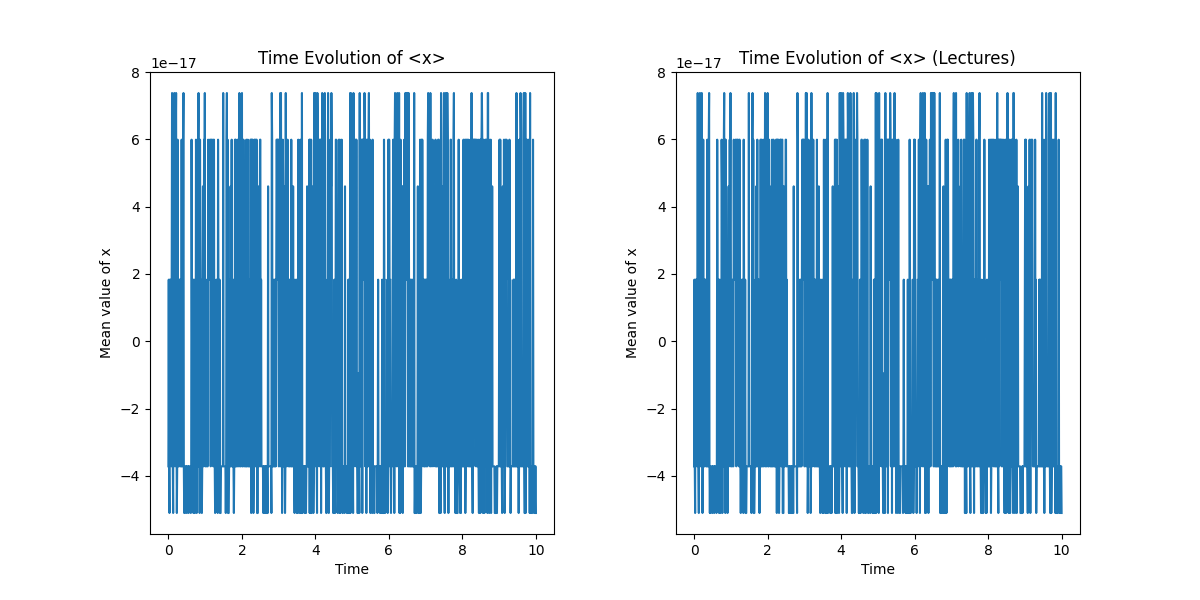
\includegraphics[scale = 0.6]{Figure_2.png}\\ 
        \end{figure}
        Η κατανομή της πιθανότητα για την χρονικη στιγμη $t=0$ θα είναι
        \begin{figure}[H]

            \centering
            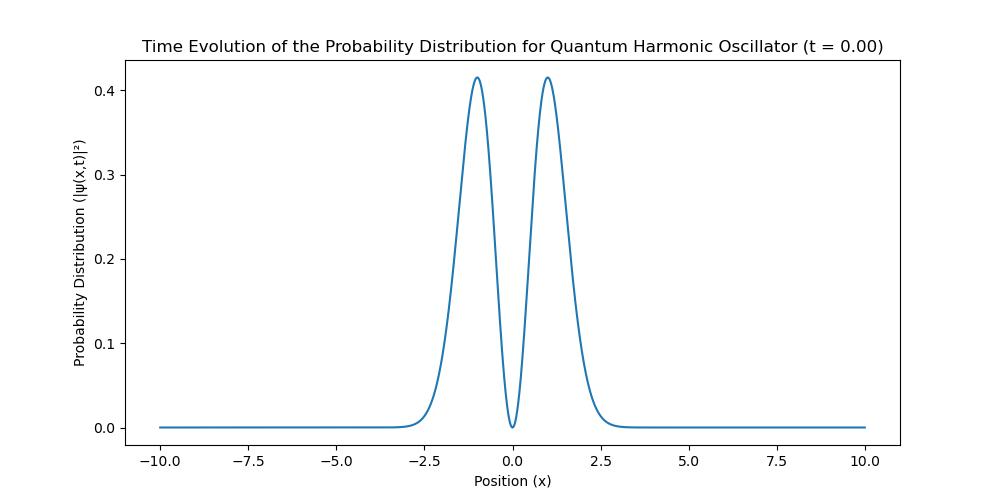
\includegraphics[scale = 0.4]{a9f29996c98e4dbf90e190930b368a61R99Q4ZKhAa9Fk3jX-0.png}\\ 
        \end{figure}
        \item για $\psi(t=0) = \frac{1}{sqrt{2}}(\ket{5}+\ket{6})$
        Η μέση τίμη της θέση σε συνάρτηση με τον χρόνο είναι
        \begin{figure}[H]

            \centering
            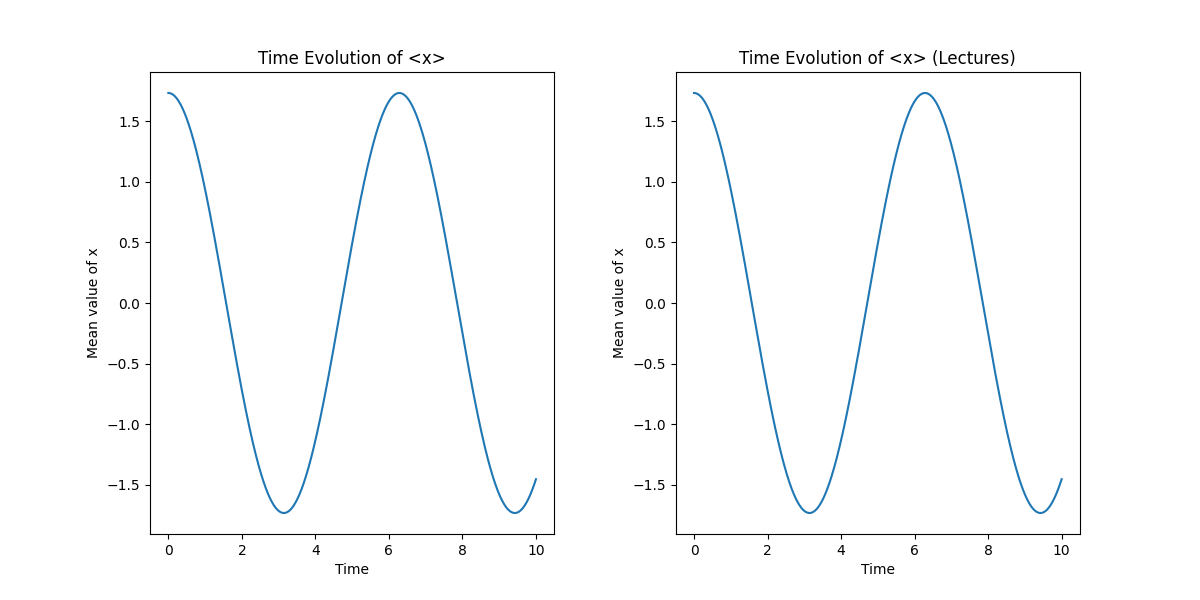
\includegraphics[scale = 0.6]{Figure_1.png}\\ 
        \end{figure}
        Η κατανομή της πιθανότητα για την χρονικη στιγμη $t=0$ θα είναι
        \begin{figure}[H]

            \centering
            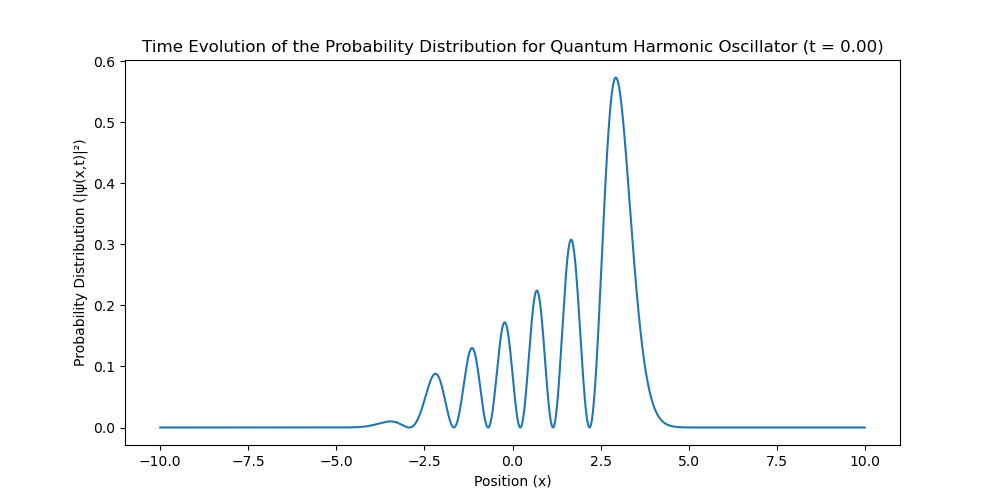
\includegraphics[scale = 0.4]{quantum_harmonic_oscillator_superpos5_6.png}\\ 
        \end{figure}
        \item για $\psi(t=0) = \frac{1}{sqrt{3}}(\ket{0}+\ket{1}+\ket{2})$
        Η μέση τίμη της θέση σε συνάρτηση με τον χρόνο είναι
        \begin{figure}[H]

            \centering
            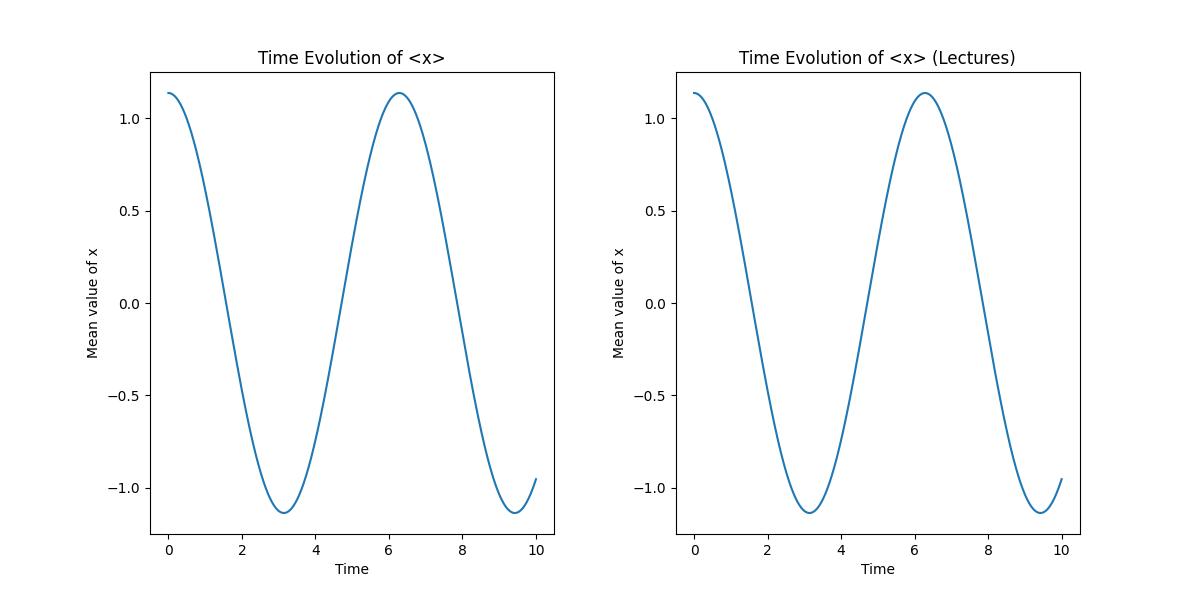
\includegraphics[scale = 0.6]{Figure_3.png}\\ 
        \end{figure}
        Η κατανομή της πιθανότητα για την χρονικη στιγμη $t=0$ θα είναι
        \begin{figure}[H]

            \centering
            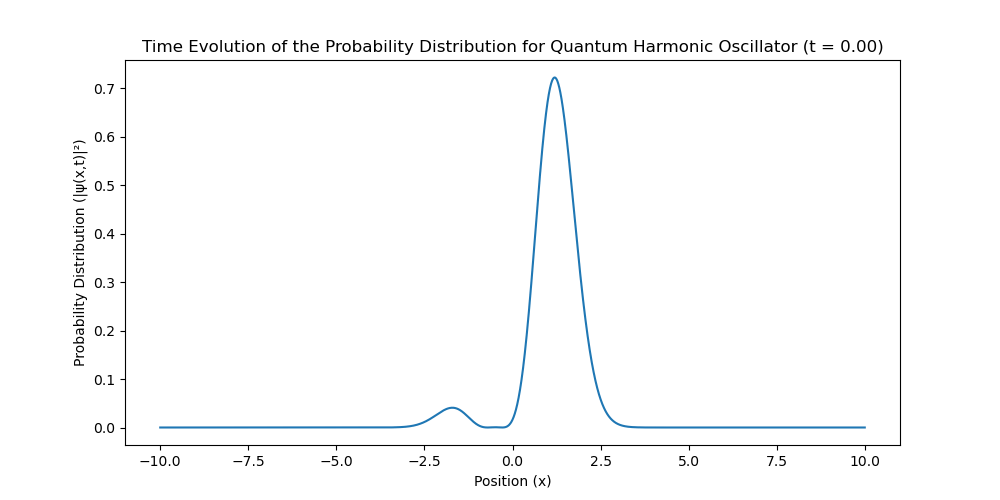
\includegraphics[scale = 0.4]{1cfa701a935b4a9bb40477fd0d2ea1bbihXSCj8JTtwuve0d-0.png}\\ 
        \end{figure}

        %\animategraphics[width=0.5\textwidth]{24}{1cfa701a935b4a9bb40477fd0d2ea1bbihXSCj8JTtwuve0d-}{0}{954}
\end{enumerate}
\end{document}